\documentclass[UTF8]{ctexbeamer}
\usepackage{latexsym}
\usepackage{amsmath,amssymb}
\usepackage{color,xcolor}
\usepackage{graphicx}
\usepackage{algorithm,listings}
\usepackage{amsthm}
\usepackage{tikz-cd}

\newcommand{\fontsm}{\fontsize{8}{9.2}\selectfont}

% \newtheorem{example}[theorem]{例} %*去除编号

\usetheme{AnnArbor}
\usefonttheme[onlymath]{serif}
\usecolortheme{crane}

\title{C语言理论题讲解}
\subtitle{Week 18}

\author[chhzh123]{陈鸿峥}
\date[Jan, 2019]{January, 2019}

\keywords{}

\begin{document}

\begin{frame}
\titlepage
\end{frame}

\begin{frame}
\tableofcontents[subsectionstyle=show]
\end{frame}

\section{在线测试}
\begin{frame}
\sectionpage
\end{frame}

\begin{frame}{在线测试}
\begin{itemize}
	\item 时间:10:00-11:00
	\item 共50道题,满分250,能做多少做多少
	\item 题目大部分原创,部分修改自sanfoundry的题目,描述均为全英
	\item 禁止使用C编译器,为避免误打误撞,本测试主要以填空题为主,若无特殊说明则直接填写程序输出
	\item 对于特殊的情况:程序编译错误请填写CE,运行时错误请填写RE,未定义行为请填写UB,无输出请填写NOTHING(注意全是大写)
	\item 注意不要输入多余空格或其他字符,注意大小写
\end{itemize}
\end{frame}

\section{讲评}
\begin{frame}
\sectionpage
\end{frame}

\begin{frame}{Q1-Q12}
前12题请翻阅上次课件\\
名词解释:
\begin{itemize}
	\item Q1: objective file: 目标文件
	\item Q3: macro: 宏
	\item Q8: 4-bit two's complement: 4位补码
\end{itemize}
\end{frame}

\begin{frame}[fragile]{Q13}
\begin{lstlisting}
#include<stdio.h>
int main()
{
    int i;
    for (i = 0; i < 10; i++)
        int b = 1;
    printf("%d",b);
}
\end{lstlisting}
b不在作用域,编译报错(CE)
\end{frame}

\begin{frame}[fragile]{Q14}
\fontsm
\begin{lstlisting}
#include<stdio.h>
int main()
{
    int i;
    extern int b;
    {
    for (i = 0; i < 10; i++)
        i++;
        int b = 10;
    }
    printf("%d %d",b,i);
    return 0;
}

int b;
\end{lstlisting}
内部b不在循环体内,但只在中间的大括号作用域内\\
printf内的b看的是外部变量b,因其为全局变量,默认初始化为0\\
i++只会影响循环次数,不会影响最终结果
\end{frame}

\begin{frame}[fragile]{Q15}
\begin{lstlisting}
#include<stdio.h>
int foo (){
    static int a;
    a++;
}

int main()
{
    int i;
    for (i = 0; i < 10; ++i)
        foo();
    printf("%d",a);
}
\end{lstlisting}
就算是static变量,作用域也是函数内部,CE
\end{frame}

\begin{frame}[fragile]{Q16}
\begin{lstlisting}
#include<stdio.h>
int foo (){
    static int a;
    auto b = 5;
    a++; b++;
    printf("%d %d ", a, b);
}

int main()
{
    int i;
    for (i = 0; i < 2; ++i)
        foo();
}
\end{lstlisting}
静态变量与自动变量\quad1 6 2 6 (space!)
\end{frame}

\begin{frame}{Q17-Q20}
见上次课件
\end{frame}

\begin{frame}{Q21}
sizeof(long) is \_\_\_\_\_ and sizeof(double) is \_\_\_\_\_ when the program is compiled by 64-bit compiler for 32-bit machine. (Enter two integers. Please separate these two numbers by ONE space)\\
\bigskip
4 8\\
sizeof编译时计算的,主要看编译器编译的对象机器
\end{frame}

\begin{frame}[fragile]{Q22}
\fontsm
\begin{lstlisting}
#include<stdio.h>
struct point
{
    int index;
    double x,y;
};

union data
{
    int index[10];
    point p[5];
};

int main()
{
    point p; data d;
    printf("%d %d", sizeof(p),sizeof(d));
}
\end{lstlisting}
忘加关键字了,以及是64位机...24 120,涉及到对齐问题,详情可见\footnote{\url{https://stackoverflow.com/questions/119123/why-isnt-sizeof-for-a-struct-equal-to-the-sum-of-sizeof-of-each-member}}
\end{frame}

\begin{frame}{Q22}
\begin{figure}
\centering
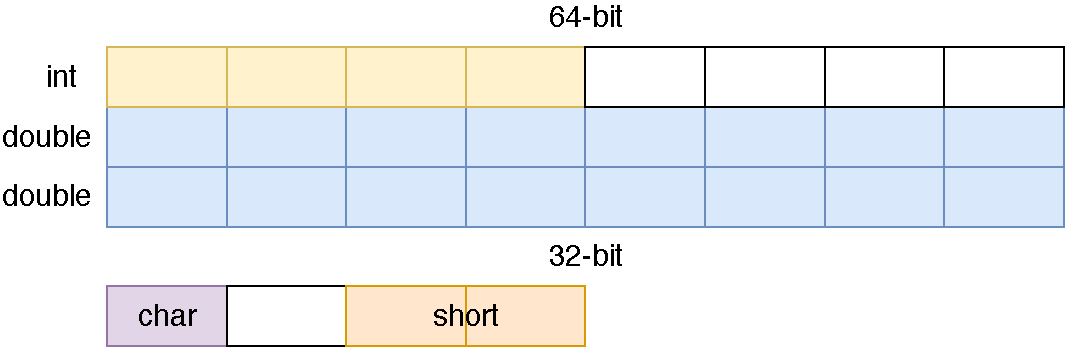
\includegraphics[width=0.8\linewidth]{fig/aligned.pdf}
\end{figure}
\end{frame}

\begin{frame}[fragile]{Q23}
\begin{lstlisting}
#include<stdio.h>
union data
{
    int index;
    char c;
}

int main()
{
    data d;
    printf("%d", sizeof(d));
}
\end{lstlisting}
分号!CE!特别留意union和struct后面!
\end{frame}

\begin{frame}{Q24-Q27}
见上次课件
\end{frame}

\begin{frame}[fragile]{Q28}
\fontsm
\begin{lstlisting}
#include <stdio.h>
int main()
{
    int ch = 1;
    switch (ch, ch + 1)
    {
    case 1:
        printf("1");
        break;
    case 2:
    case 3:
        printf("3");
        break;
    }
    return 0;
}
\end{lstlisting}
逗号表达式,取后者为2\\
case没有break往下执行,输出3
\end{frame}

\begin{frame}[fragile]{Q29}
\begin{lstlisting}
#include <stdio.h>
int main()
{
    int x = 0;
    if (x++)
        printf("true");
    else if (x = 2)
        printf("false");
    else
        printf("nothing");
}
\end{lstlisting}
第一条if,先判断为0假,x++得到1\\
第二条if,等号赋值x为2,非零值为真,输出false
\end{frame}

\begin{frame}[fragile]{Q30}
\begin{lstlisting}
#include <stdio.h>
    int main()
    {
        int a = 1;
        if (a)
            printf("A");
            printf("B");
        else
            printf("C");
    }
\end{lstlisting}
CE,千万不要被缩进误导!
\end{frame}

\begin{frame}[fragile]{Q31}
\begin{lstlisting}
#include <stdio.h>
int main()
{
    if (printf("0"))
        printf("1");
    else
    	printf("0");
}
\end{lstlisting}
01\\
printf和scanf都有返回值,字符类型非0为真
\end{frame}

\begin{frame}[fragile]{Q32}
\begin{lstlisting}
#include <stdio.h>
int main()
{
    int x = 0;
    if (++x || ++x || x++)
        printf("%d", x);
}
\end{lstlisting}
1\\
与或都有短路特性
\end{frame}

\begin{frame}{Q33-Q34}
见上次课件
\end{frame}

\begin{frame}[fragile]{Q35}
\begin{lstlisting}
What is the output of this C code?
#include <stdio.h>
int main()
{
    int y = 1, x = 0;
    int l = (y++, x++) ? y : x;
    printf("%d", l);
}
\end{lstlisting}
1\\
逗号表达式结合自增、三目运算符\\
注意后自增是在\textbf{括号表达式执行完}就自增了
\end{frame}

\begin{frame}[fragile]{Q36-Q37}
Q36: for循环三个分号一个都不能少\\
Q37: 奇怪的for循环也是可以执行的
\begin{lstlisting}
#include <stdio.h>
int main()
{
    int i = 0;
    for (i++; i == 1; i = 2)
        printf("A");
        printf("B");
}
\end{lstlisting}
\begin{itemize}
	\item 初始化i为0,之后自增为1
	\item 循环体输出A
	\item 执行赋值操作i=2
	\item 判断条件i==1不成立,跳出循环,输出B
\end{itemize}
\end{frame}

\begin{frame}{Q38-40}
运算符优先级,见上次课件\\
\begin{center}
\Large\textbf{单算移关与,异或逻条赋}
\end{center}
\end{frame}

\begin{frame}[fragile]{Q41}
\begin{lstlisting}
foo()
{
    return (double)(char)5.0;
}
\end{lstlisting}
可以执行多个类型转换,同时注意默认为无返回类型的函数默认为int,若是void要明确指出
\end{frame}

\begin{frame}{Q42-43}
见上次课件,常量指针与指针常量
\end{frame}

\begin{frame}{Q44}
sizeof指针只关心机器字长
\end{frame}

\begin{frame}[fragile]{Q45}
\fontsm
\begin{lstlisting}
#include <stdio.h>
int myfoo(int);
int (*fooptr)(int);
int (*foo(int))(int);

int main(){
    fooptr = foo(0);
    fooptr(10);
}
int (*foo(int i))(int){
    return myfoo;
}
int myfoo(int i){
    printf("%d", i + 1);
}
\end{lstlisting}
全卷最绕一题,11\\
fooptr为一个形参为int返回值为int的函数的指针\\
foo为一个形参为int返回值为【形参为int返回值也为int的函数的指针】的函数\\
foo(int) $\to$ *(foo(int)) $\to$ int (*(foo(int)))(int)\\
myfoo即为这样的函数
\end{frame}

\begin{frame}{Q46-Q47}
Q46: int *p=0就是空指针\\
Q47: 见上次课件,二重指针
\end{frame}

\begin{frame}[fragile]{Q48}
\begin{lstlisting}
#include <stdio.h>
int main()
{
    int arr[3][4] = {5,6,7,8,9,10};
    printf("%d", 1[arr][0]);
}
\end{lstlisting}
二维数组初始化可以不写内层括号,可以只初始化前面的元素\\
原式等价于\verb'arr[3][4] = {{5,6,7,8},{9,10,0,0},...}'\\
1[arr]等价于arr[1],故访问第1行第0个元素,即为9
\end{frame}

\begin{frame}{Q49-Q50}
Q49: 见上次课件,指针负索引,printf补零\\
Q50: 见上次课件,Linux操作,注意dir是windows命令行的操作
\end{frame}

\begin{frame}{总结}
\begin{itemize}[<+->]
	\item 真正考试一定不会出这些题
	\item 还要多刷题,最好把题库刷穿
	\item 祝大家考试顺利!
\end{itemize}
\end{frame}

\end{document}